\documentclass[a4paper]{article}

%% Language and font encodings
\usepackage[english]{babel}
\usepackage[utf8x]{inputenc}
\usepackage[T1]{fontenc}

%% Sets page size and margins
\usepackage[a4paper,top=3cm,bottom=2cm,left=3cm,right=3cm,marginparwidth=1.75cm]{geometry}

%% Useful packages
\usepackage{amsmath}
\usepackage{graphicx}
\usepackage[colorinlistoftodos]{todonotes}
\usepackage[colorlinks=true, allcolors=blue]{hyperref}
\usepackage{alltt}

\title{Reporte de Evaluación2}
\author{Valenzuela Terán Jonás}

\begin{document}
\maketitle

\begin{center}
	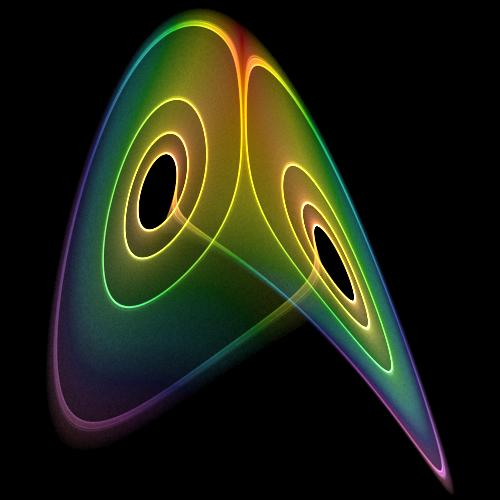
\includegraphics[height=8cm]{Intermittent_Lorenz_Attractor_-_Chaoscope.jpg}
\end{center}


\section{Introducción}

El objetivo de la evaluación es poner a prueba conocimientos previos sobre manejo de modelos en python, en el entorno de programación jupyter lab, además de manejo de herramientas de graficación y solucionadores numéricos. Además, se aprenderá a crear un GIF animado del modelo, usando como ejemplo el sistema de Lorenz, ilustrando el espacio de fase (posición contra posición) que produce con diferentes parámetros definidos.


\section{Sistema de Lorenz}

El sistema de Lorenz es un sistema de ecuaciones diferenciales ordinarias, estudiadas por Edward Lorenz, es característica por tener soluciones caóticas con ciertos valores de parámetros y condiciones iniciales, estas soluciones muestran gráficas de fase con figuras de mariposa o de infinito comunmente.

\begin{center}
$\frac{dx}{dt} = \sigma (y - x)$

$\frac{dy}{dt} = x(\rho - z) - y$

$\frac{dz}{dt} = xy - \beta z$
\end{center}

Esto se conoce como las ecuaciones de Lorenz, se relacionan con una simplificación del modelo matemático de convección atmosférica, las propiedades de una capa de fluido bi-dimensional uniformemente calentado desde abajo y enfriado desde arriba. Edward Lorenz, considerado el padre de la teoría del caos, describió el caos una vez como: “cuando el presente determina el futuro, pero el presente aproximado no determina aproximadamente el futuro”.

\section{Resultados}

En el primer caso, exploramos el sistema de Lorenz con parámetros: $\sigma = 10, \beta = \frac{8}{3}, \rho = 28$.

\begin{center}
	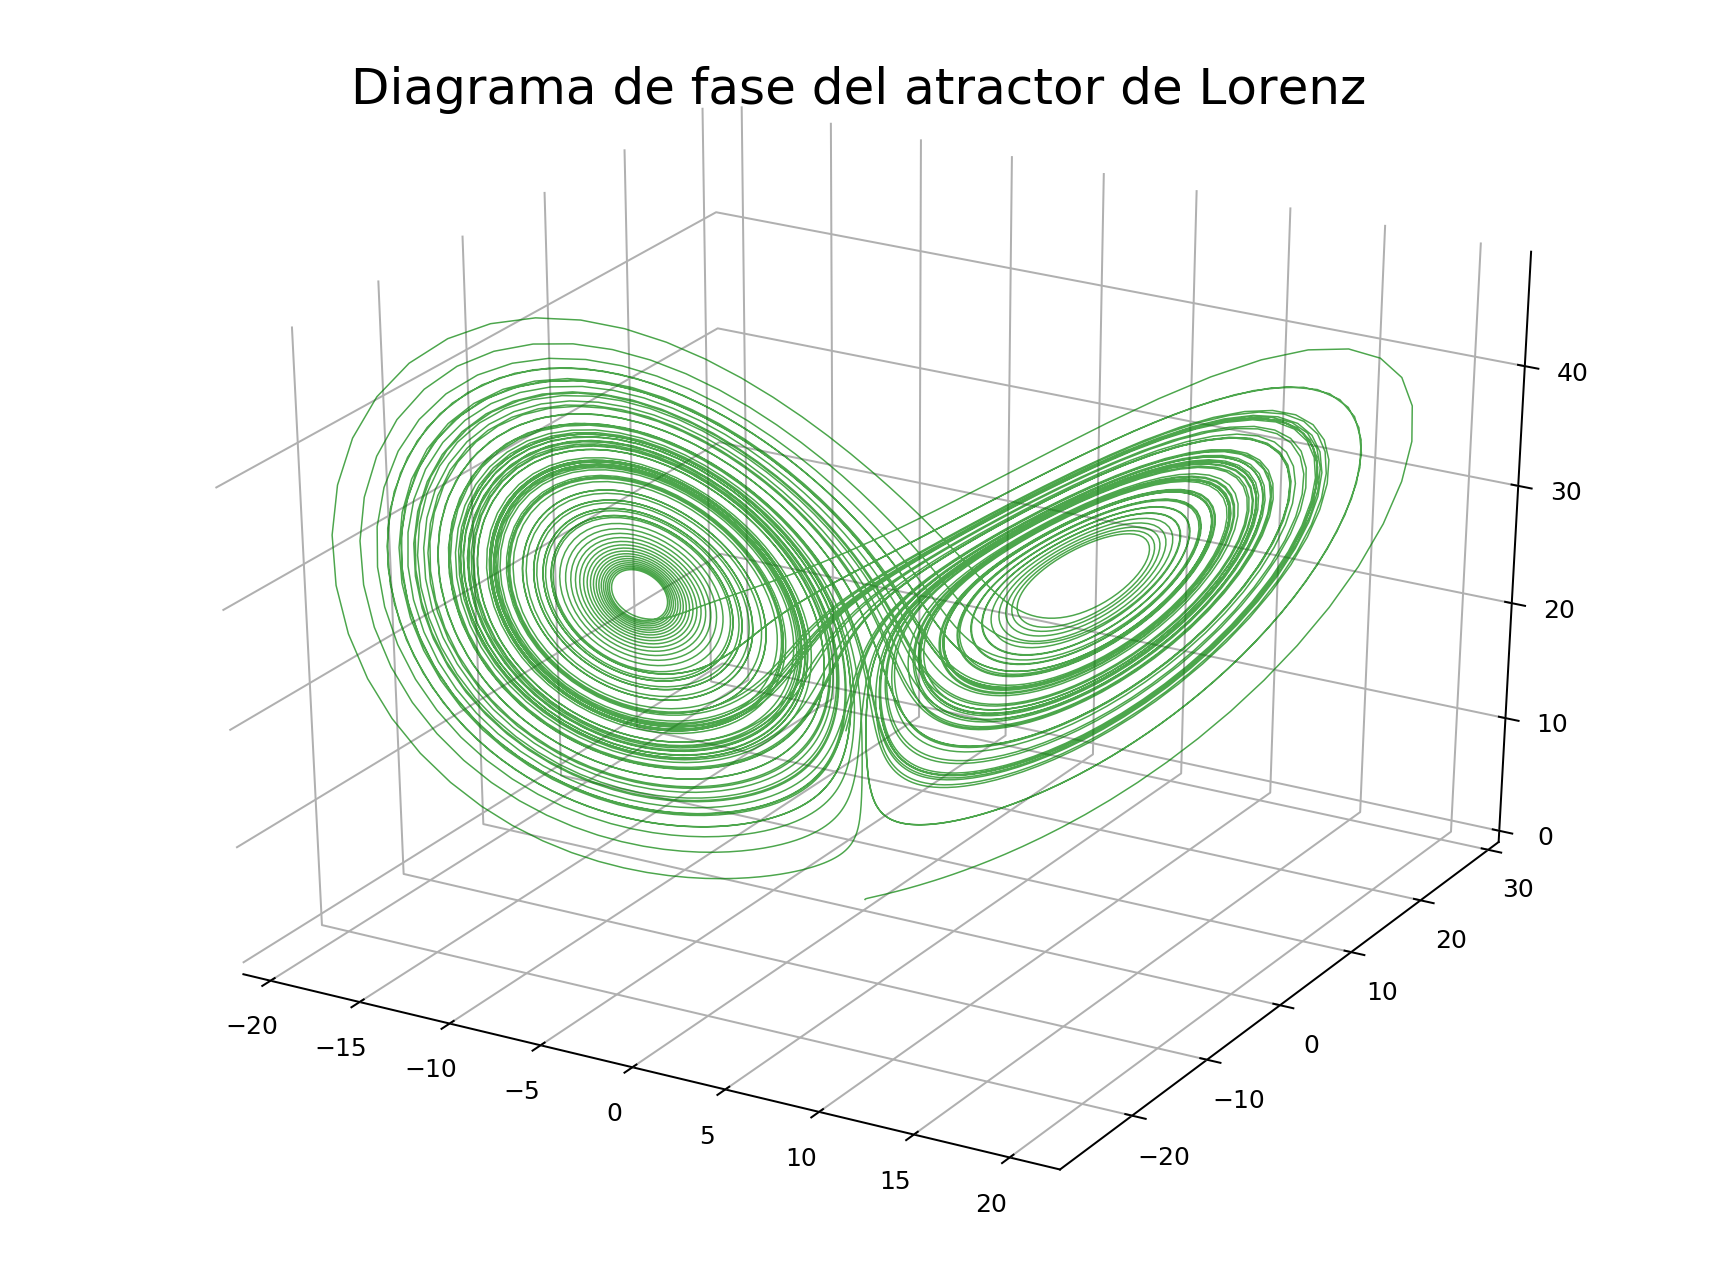
\includegraphics[height=5cm]{lorenz-attractor-3d1.png}
\end{center}

Primero realizamos una gráfica de fase en el espacio, con las coordenadas $x, y, z$ se forma una figura similar a una mariposa o al símbolo de infinito.

\begin{center}
	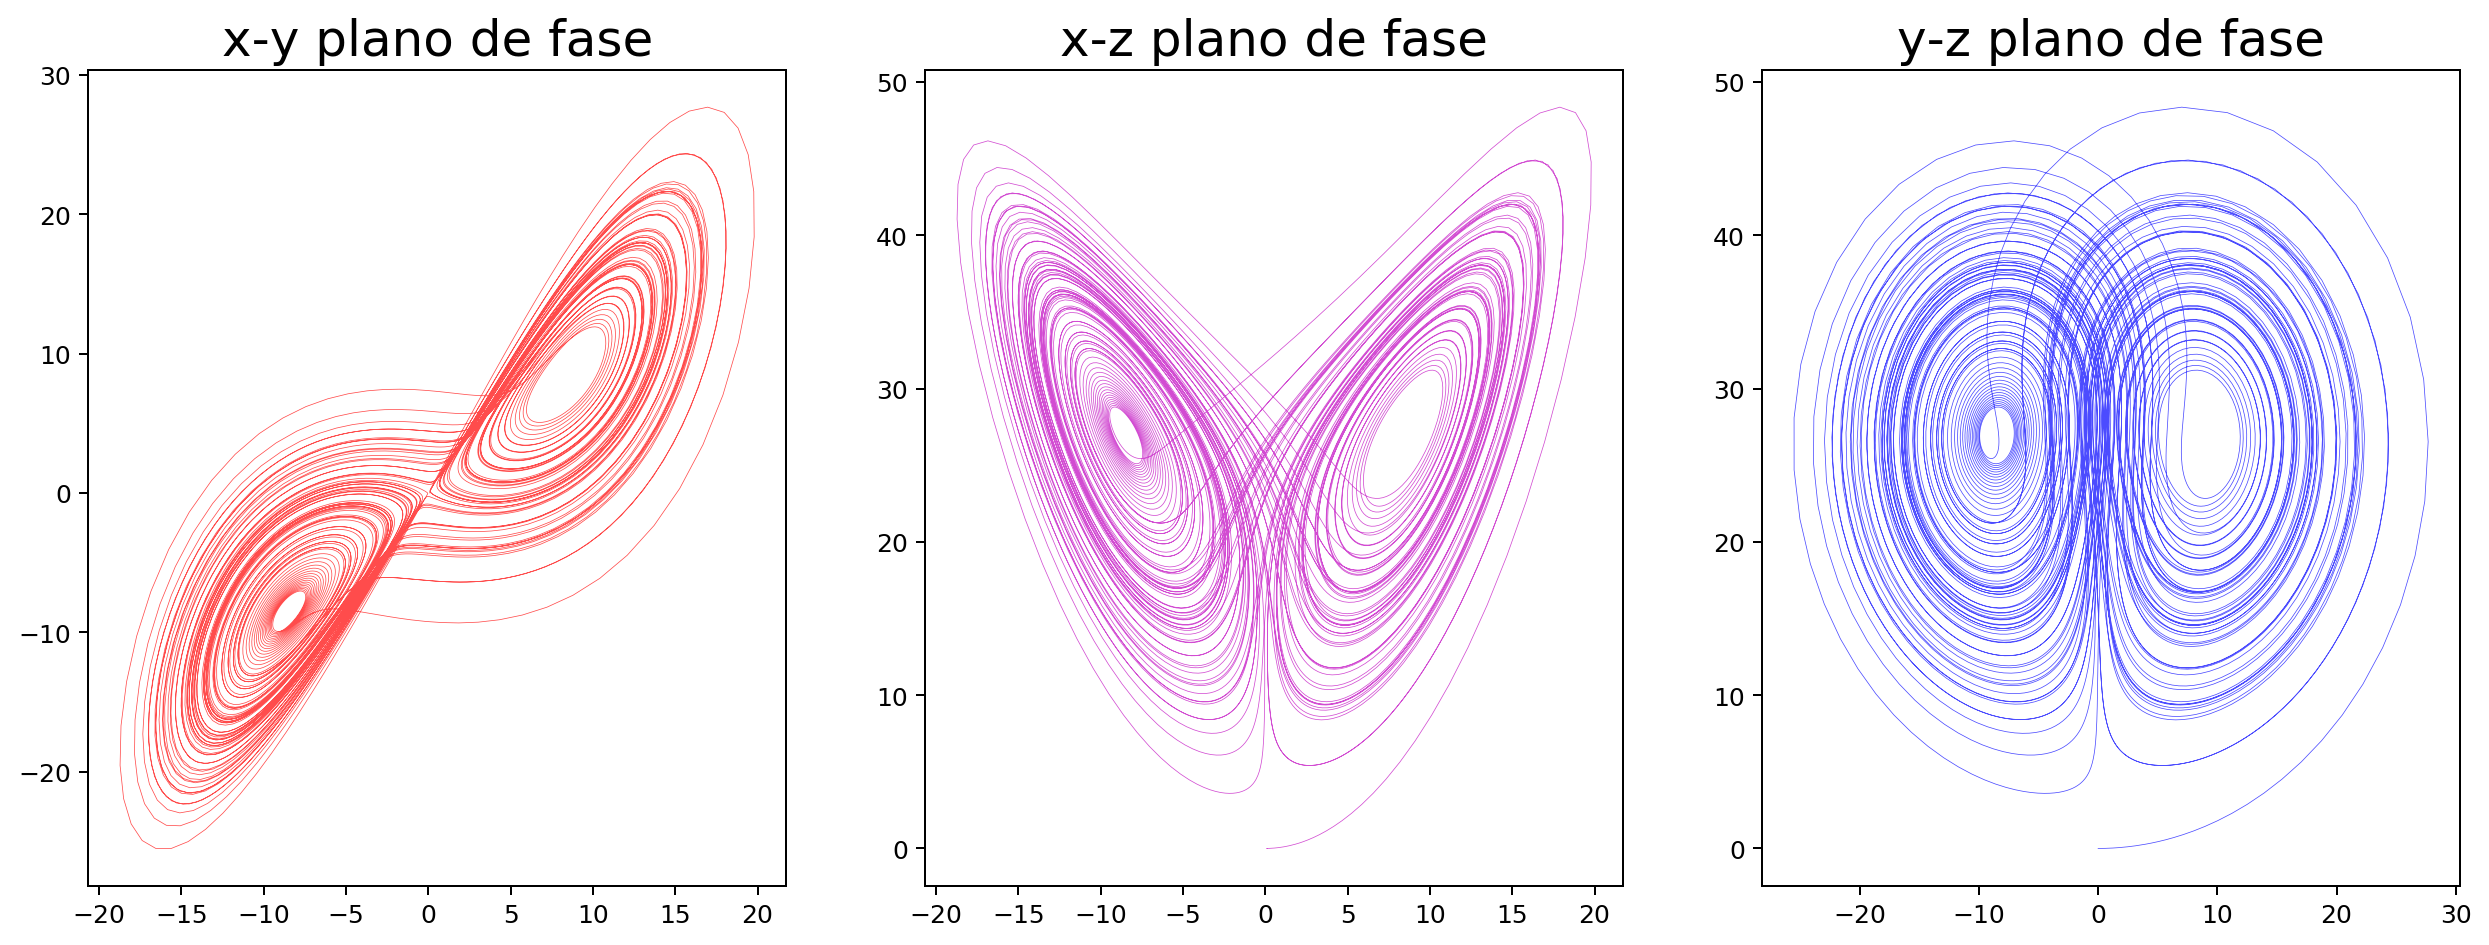
\includegraphics[height=5cm]{lorenz-attractor-phase-plane1.png}
\end{center}

Realizamos gráficas de fase bi-dimensionales para analizar más a detalle cada componente, observamos patrones similares en las 3 combinaciones.

\begin{center}
	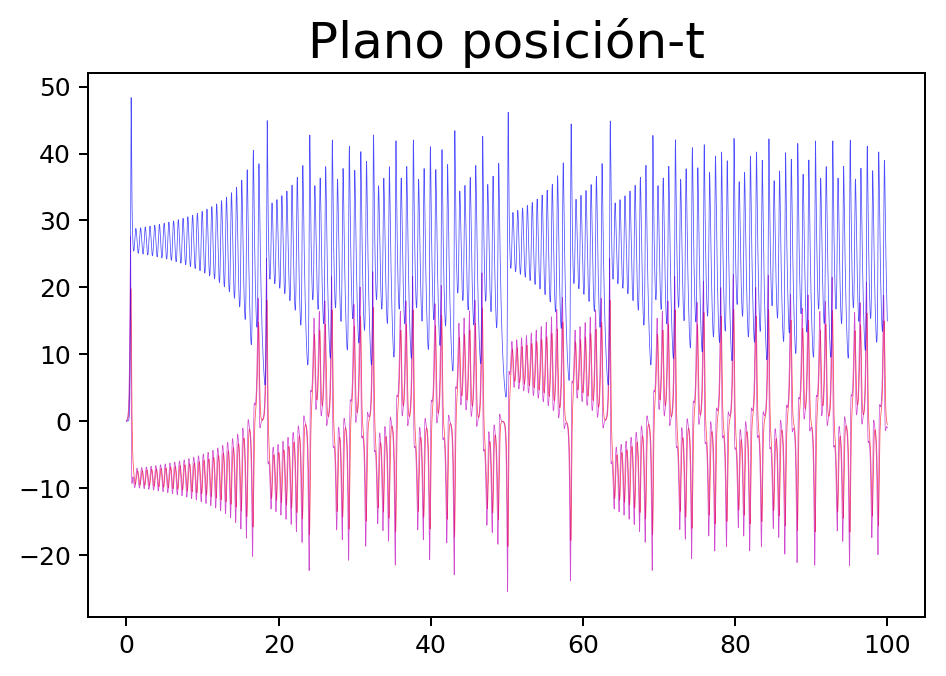
\includegraphics[height=5cm]{lorenz-attractor-xt-plane1.png}
\end{center}

Finalmente creamos una gráfica de posición contra tiempo, de $x, y, z$ superpuestas, asignadas con un color diferente, aquí se puede apreciar el comportamiento caótico del sistema.

\vspace{0.75cm}

Para el segundo caso, exploramos con los parámetros: $\sigma = 28, \beta = 4, \rho = 46.92$.

\begin{center}
	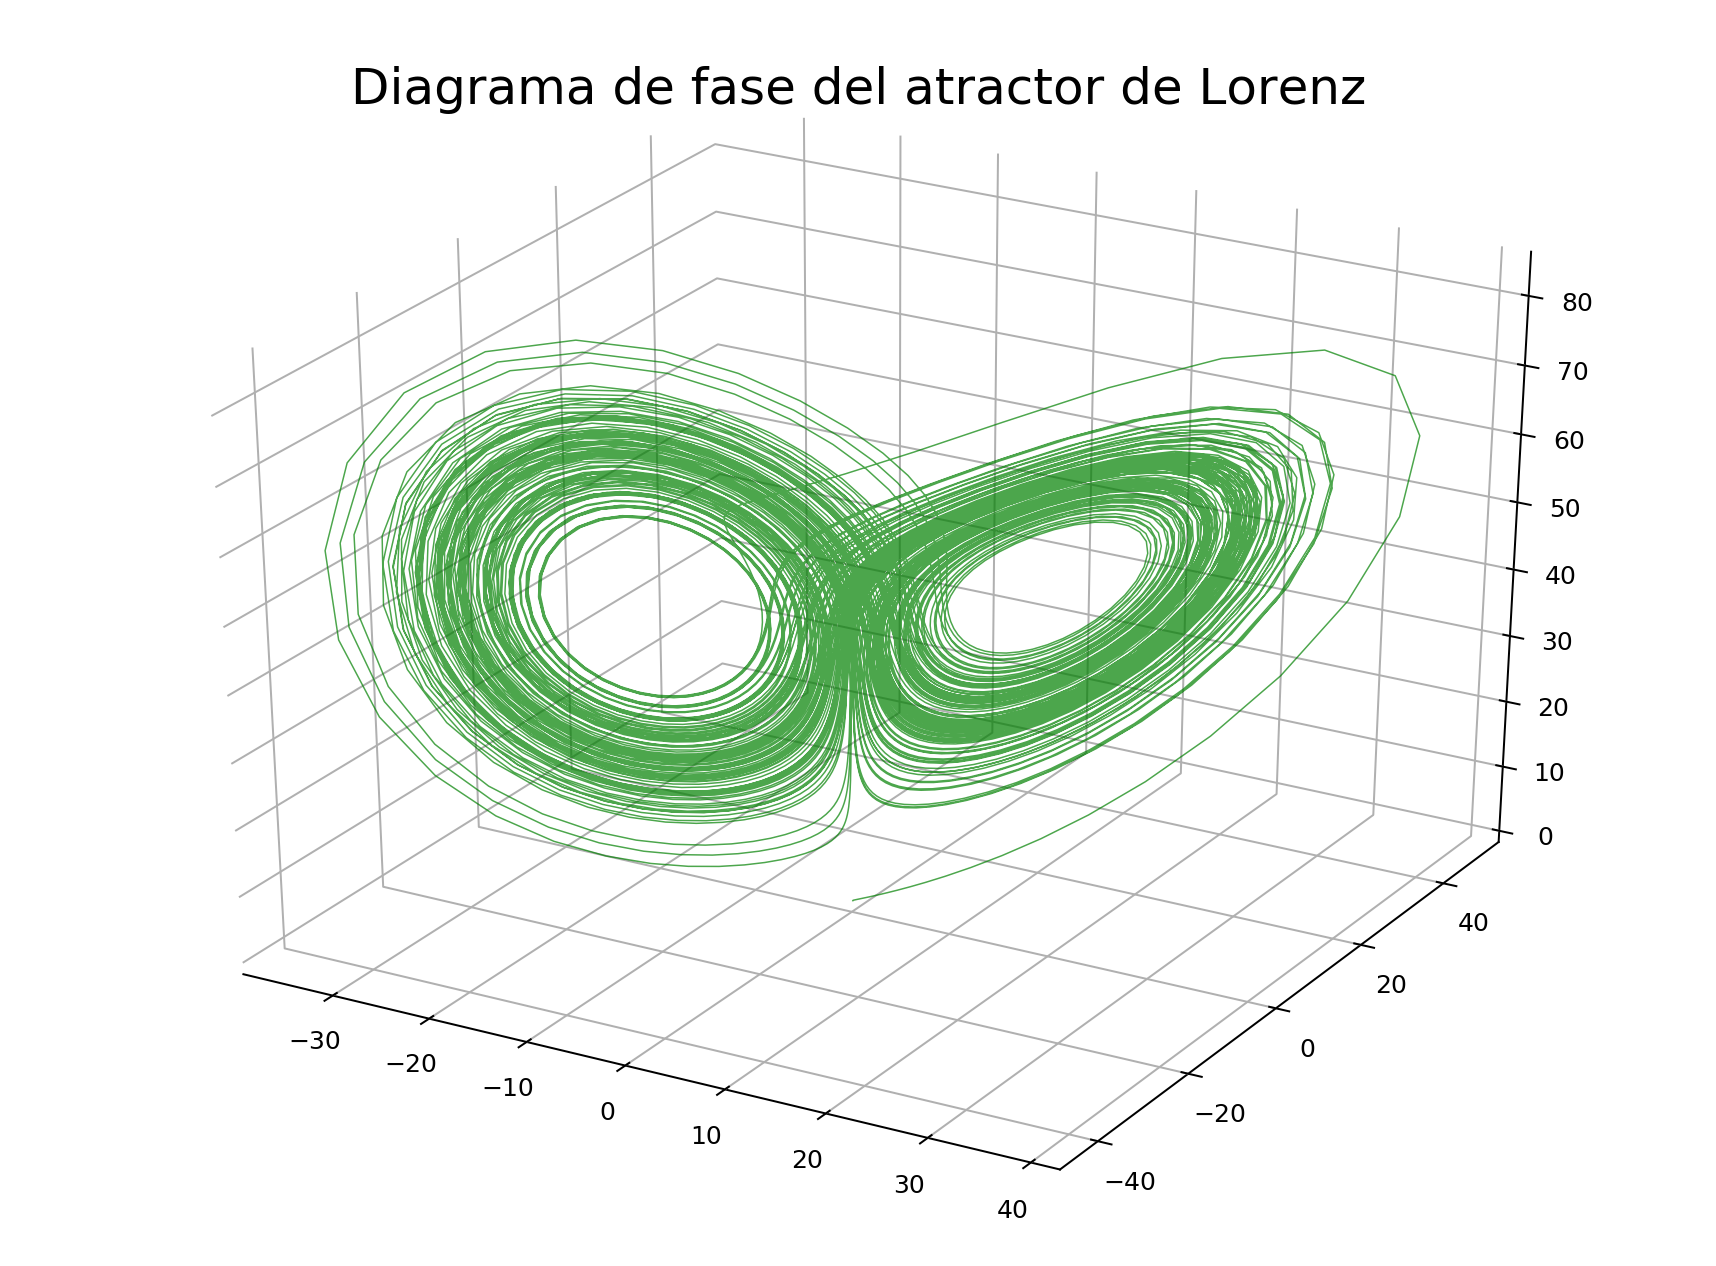
\includegraphics[height=5cm]{lorenz-attractor-3d2.png}
\end{center}

Observamos una trayectoria de fase más definida, es decir, se dispersa menos, formando un patrón más apreciable.

\begin{center}
	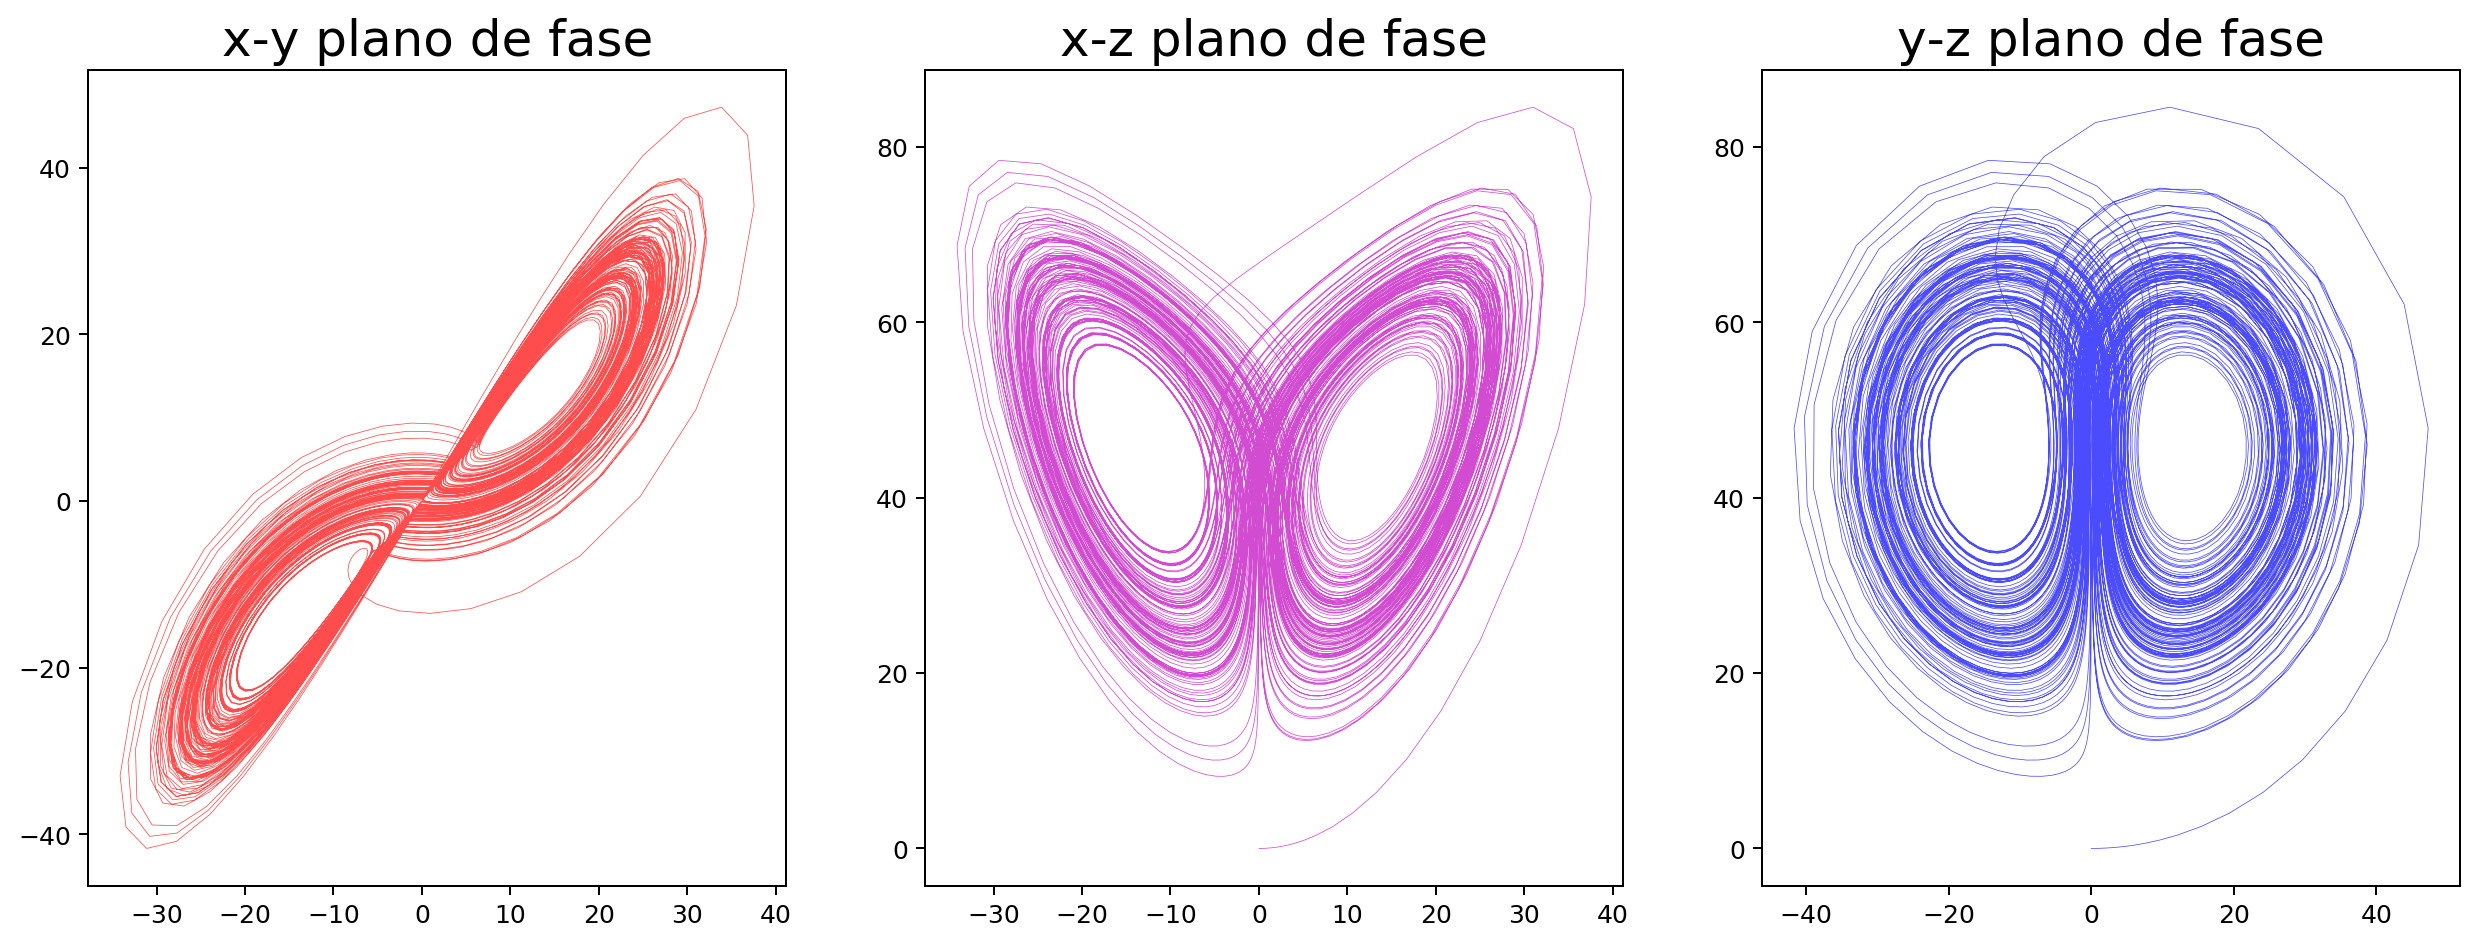
\includegraphics[height=5cm]{lorenz-attractor-phase-plane2.png}
\end{center}

En los planos de fase individuales observamos el mismo caso, las trayectorias y patrones se definen más.

\begin{center}
	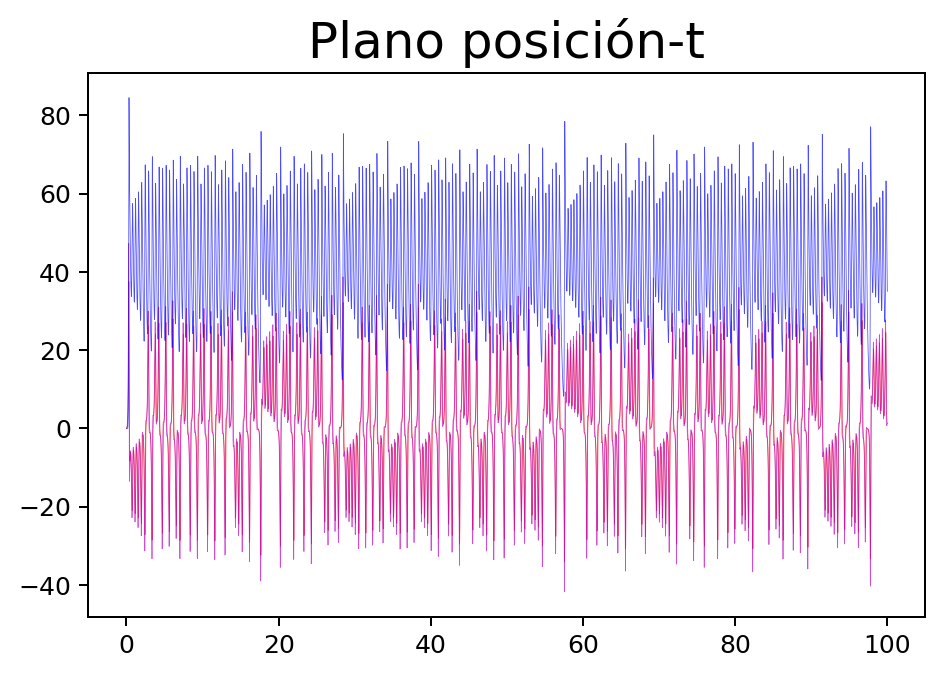
\includegraphics[height=5cm]{lorenz-attractor-xt-plane2.png}
\end{center}

La gráfica de posición contra tiempo, muestra movimientos menos caóticos, además, distinguibles entre $x, y, z$ por su posición promedio.

\vspace{0.75cm}

Finalmente, el tercer caso, considera los parámetros: $\sigma = 10, \beta = \frac{8}{3}, \rho = 99.96$.

\begin{center}
	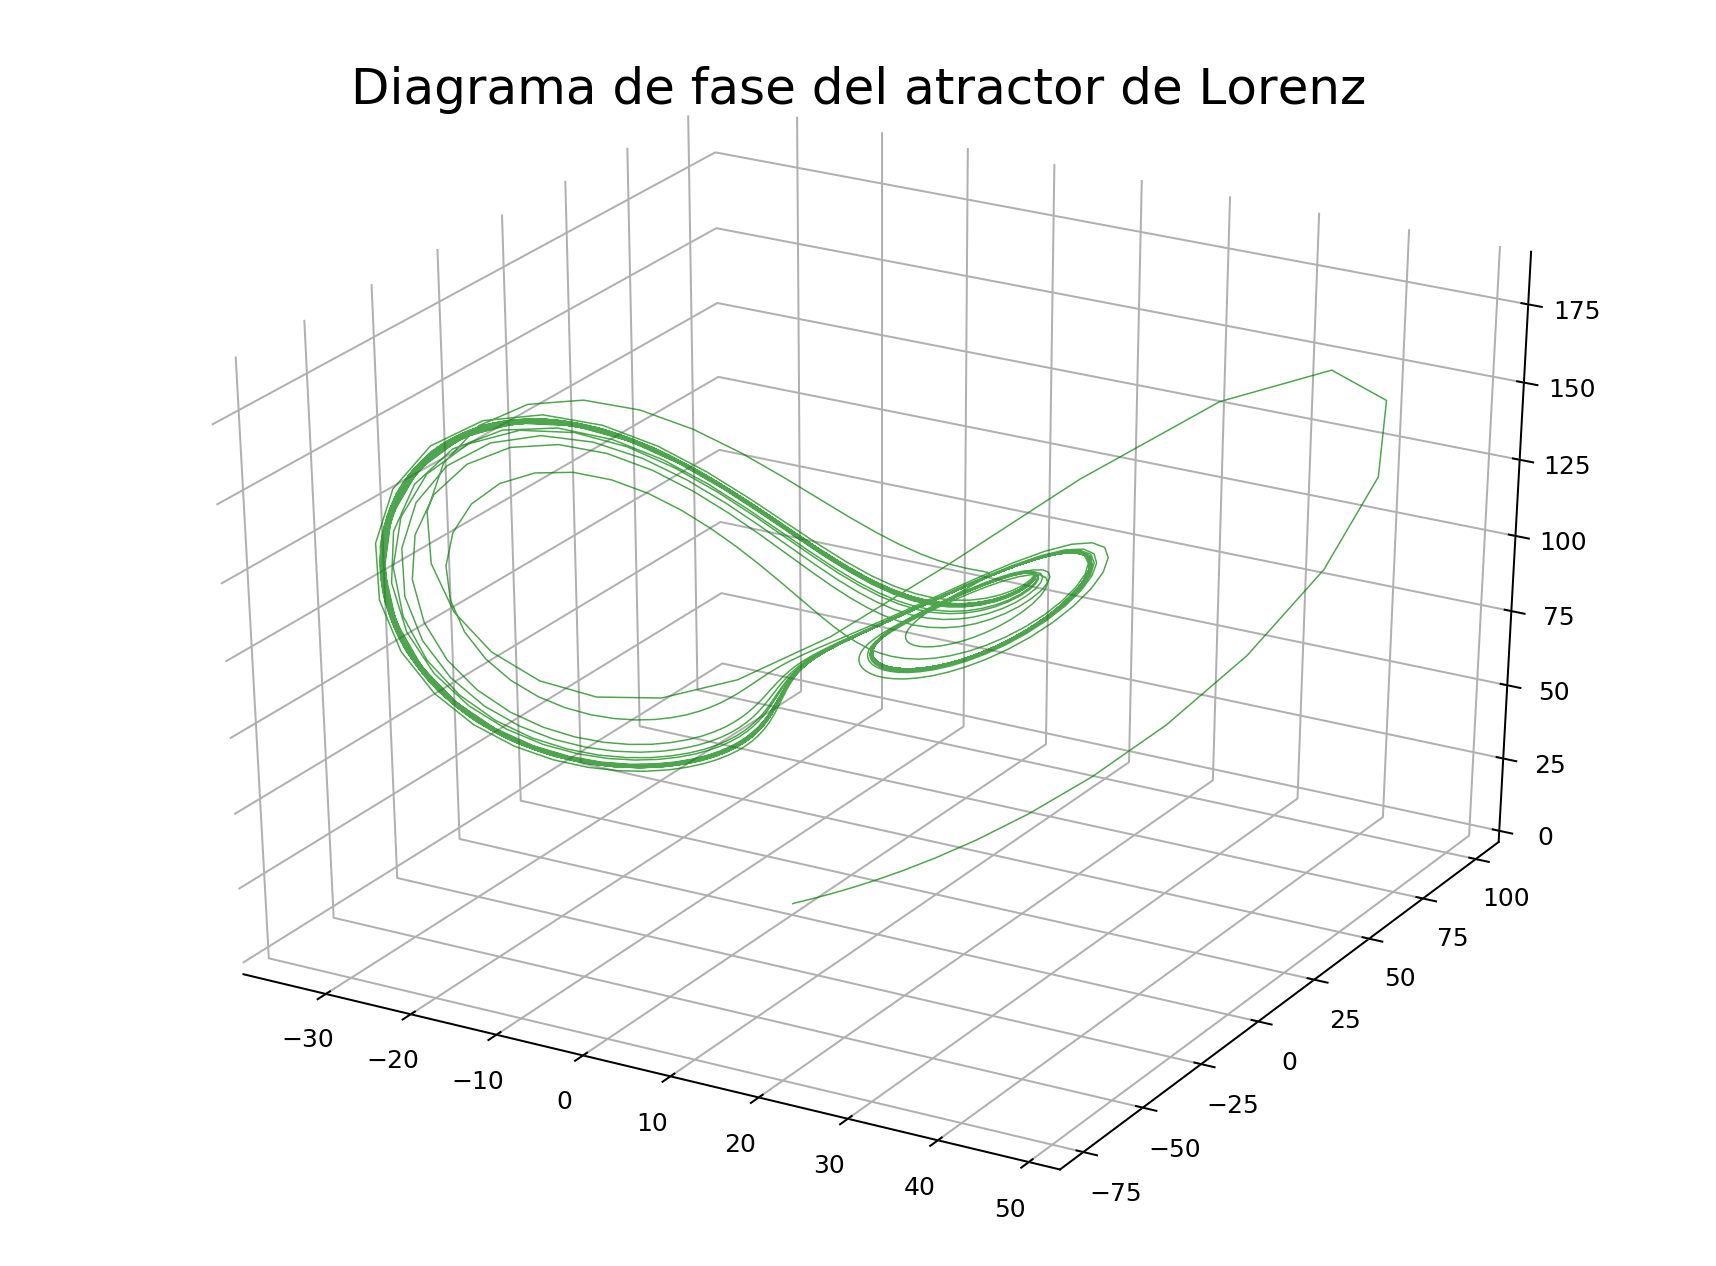
\includegraphics[height=5cm]{lorenz-attractor-3d3.png}
\end{center}

Es evidente que el espacio de fase obtenido de estos parámetros es muy diferente a los 2 anteriores, la trayectoria es mucho más definida, describiendo un ciclo límite, sin embargo, este no tiene la forma de mariposa o infinito visto anteriormente.

\begin{center}
	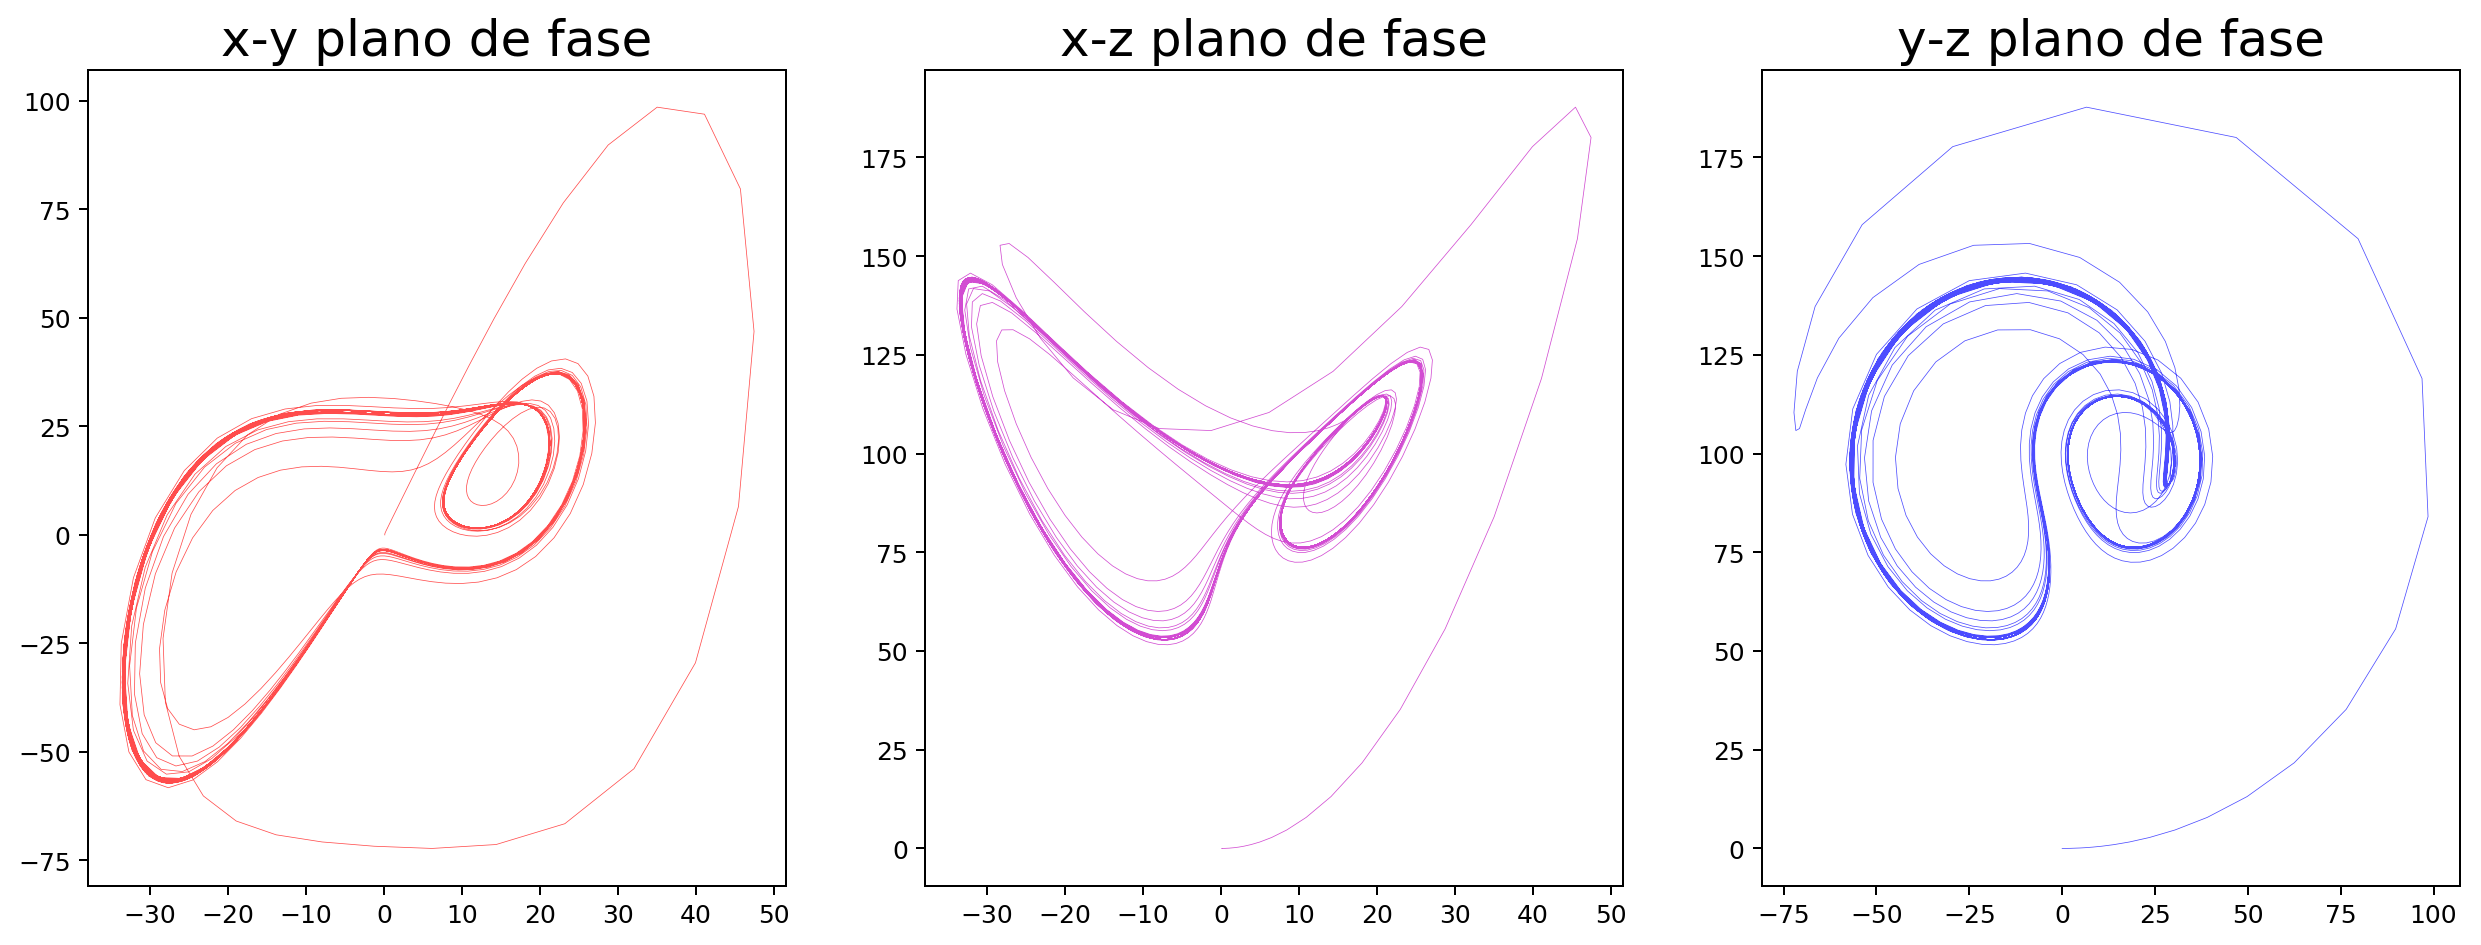
\includegraphics[height=5cm]{lorenz-attractor-phase-plane3.png}
\end{center}

Lo mismo sigue si analizamos las direcciones coordenadas individualmente, mostrando figuras irregulares pero estables y cerradas.

\begin{center}
	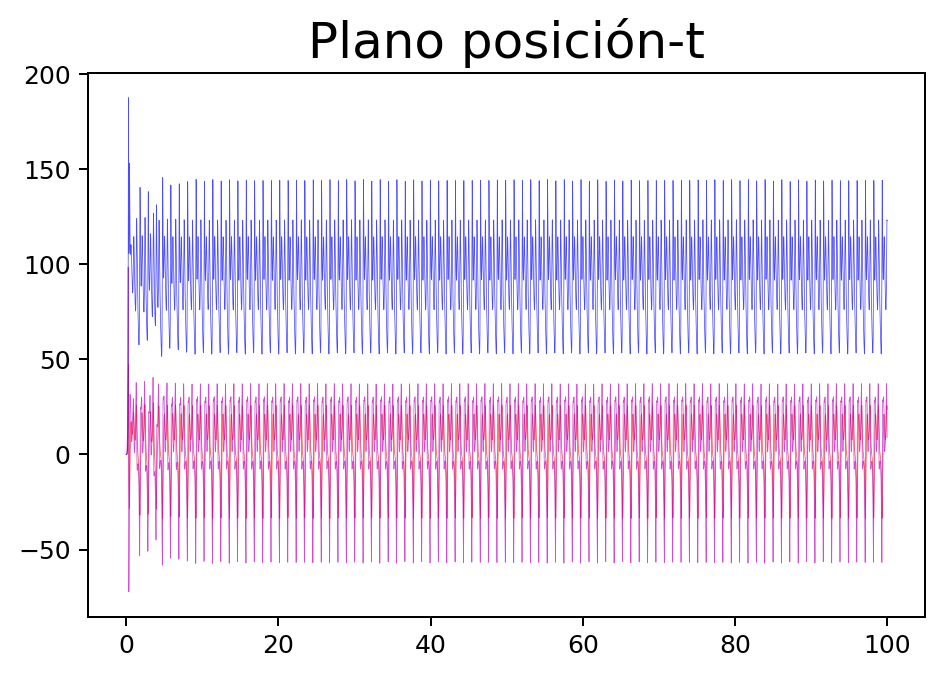
\includegraphics[height=5cm]{lorenz-attractor-xt-plane3.png}
\end{center}

Analizando el plano de posición contra tiempo, notamos la periodicidad del movimiento comparado con los movimientos anteriores, lo que demuestra que los parámetros afectan fuertemente en la solución del sistema y su comportamiento.


\section{Conclusión}

La evaluación cumplió en poner los conocimientos previos a prueba, al solucionar los posibles errores que se presentaran al tratar de reproducir el sistema de Lorenz en diferentes condiciones, además, se aprendió a realizar una animación de el modelo, que es útil para cualquier modelo, observamos también el sistema de Lorenz que produce patrones muy interesantes, un ejemplo adecuado para animar.


\section{Bibliografía}

\begin{itemize}
\item (2018). Lorenz system. 26 de abril de 2018, de Wikipedia Sitio web: 
\textit{https://en.wikipedia.org/wiki/Lorenz\_system}

\item Geoff Boeing. (2016). Animating the Lorenz Attractor with Python. 26 de abril de 2018, de Urban planning postdoc at UC Berkeley Sitio web: 
http://geoffboeing.com/2016/12/animating-lorenz-attractor-python/
\end{itemize}


\end{document}